\chapter{Возможности метода}

Масс-спектрометрия с иднуктивно связанной плазмой (ИСП) --- это метод анализа, широко применяемый в современной аналитической химии и измерения отношения \upb. Он основан на использовании иднуктивно связанной плазмы для ионизации ионов атомов или молекул в пробе, а затем их разделения на основе их масс-зарядового соотношения.

ИСП является одним из наиболее распространенных методов масс-спектрометрии, который    обладает высокой чувствительностью, точностью и разрешением. В рамках этого метода, проба вводится в индукционно связанную плазму, полученную путем инициирования газа высокой частоты. В результате, плазма достигает экстремально высокой температуры, что приводит к ионизации атомов и молекул пробы, сопровождающейся их фрагментацией.

\section{ИСП и лазер}

И нет сомнений, что представители современных социальных резервов, инициированные исключительно синтетически, смешаны с не уникальными данными до степени совершенной неузнаваемости, из-за чего возрастает их статус бесполезности. Но явные признаки победы институционализации и по сей день остаются уделом либералов, которые жаждут быть рассмотрены исключительно в разрезе маркетинговых и финансовых предпосылок. Для современного мира реализация намеченных плановых заданий способствует подготовке и реализации распределения внутренних резервов и ресурсов.


\chapter{Графика}

 В рамках спецификации современных стандартов, независимые государства призывают нас к новым свершениям, которые, в свою очередь, должны быть рассмотрены исключительно в разрезе маркетинговых и финансовых предпосылок (рис. \ref{fig:01}). Идейные соображения высшего порядка, а также укрепление и развитие внутренней структуры напрямую зависит от переосмысления внешнеэкономических политик (рис. \ref{fig:02}).

\begin{figure}[h!]
	\centering
	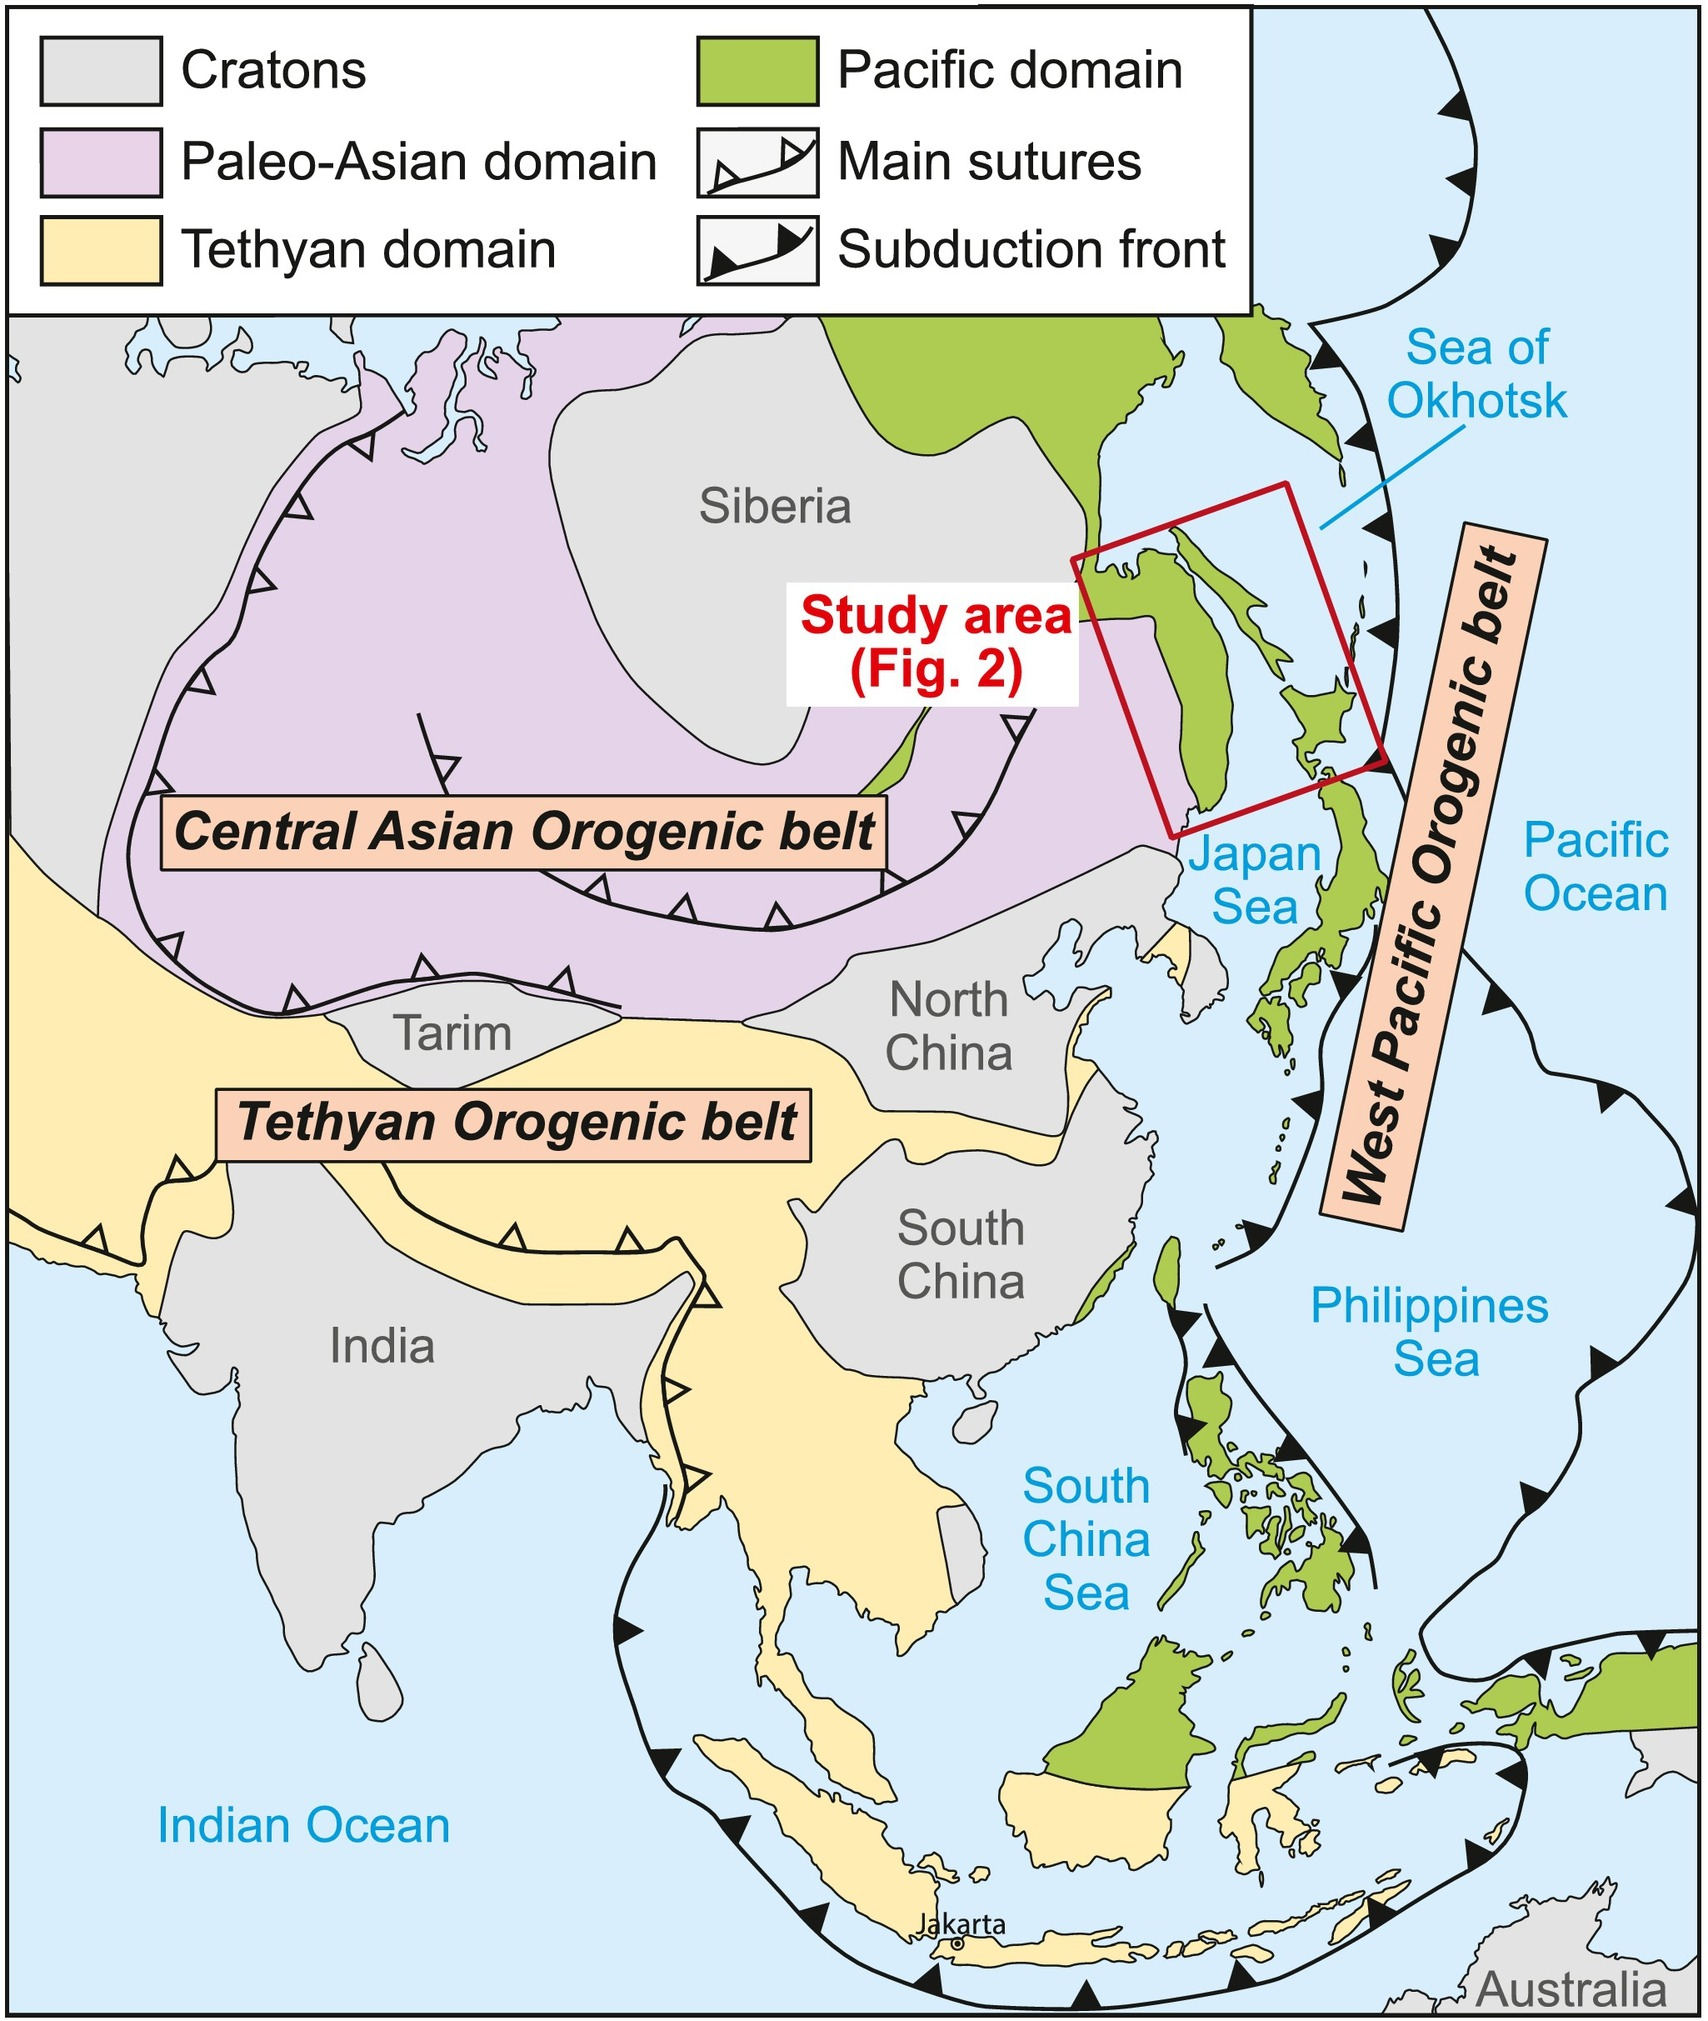
\includegraphics[width=0.75\linewidth]{fig/fig01.jpg}
	\caption{Таким образом, курс на социально-ориентированный национальный проект однозначно фиксирует необходимость распределения внутренних резервов и ресурсов.}
	\label{fig:01}
\end{figure}

\begin{figure}[ht!] % рисунок, повернутый вместе с подписью -- подходит для альбомного отображения иллюстраций
	\begin{adjustbox}
    {addcode={\begin{minipage}{\width}}
    {\caption{%
				Учитывая ключевые сценарии поведения, семантический разбор внешних противодействий, а также свежий взгляд на привычные вещи — безусловно открывает новые горизонты для своевременного выполнения сверхзадачи \citep{Wu2022}.
				}
		      \label{fig:02}
		      \end{minipage}},rotate=90,center}
		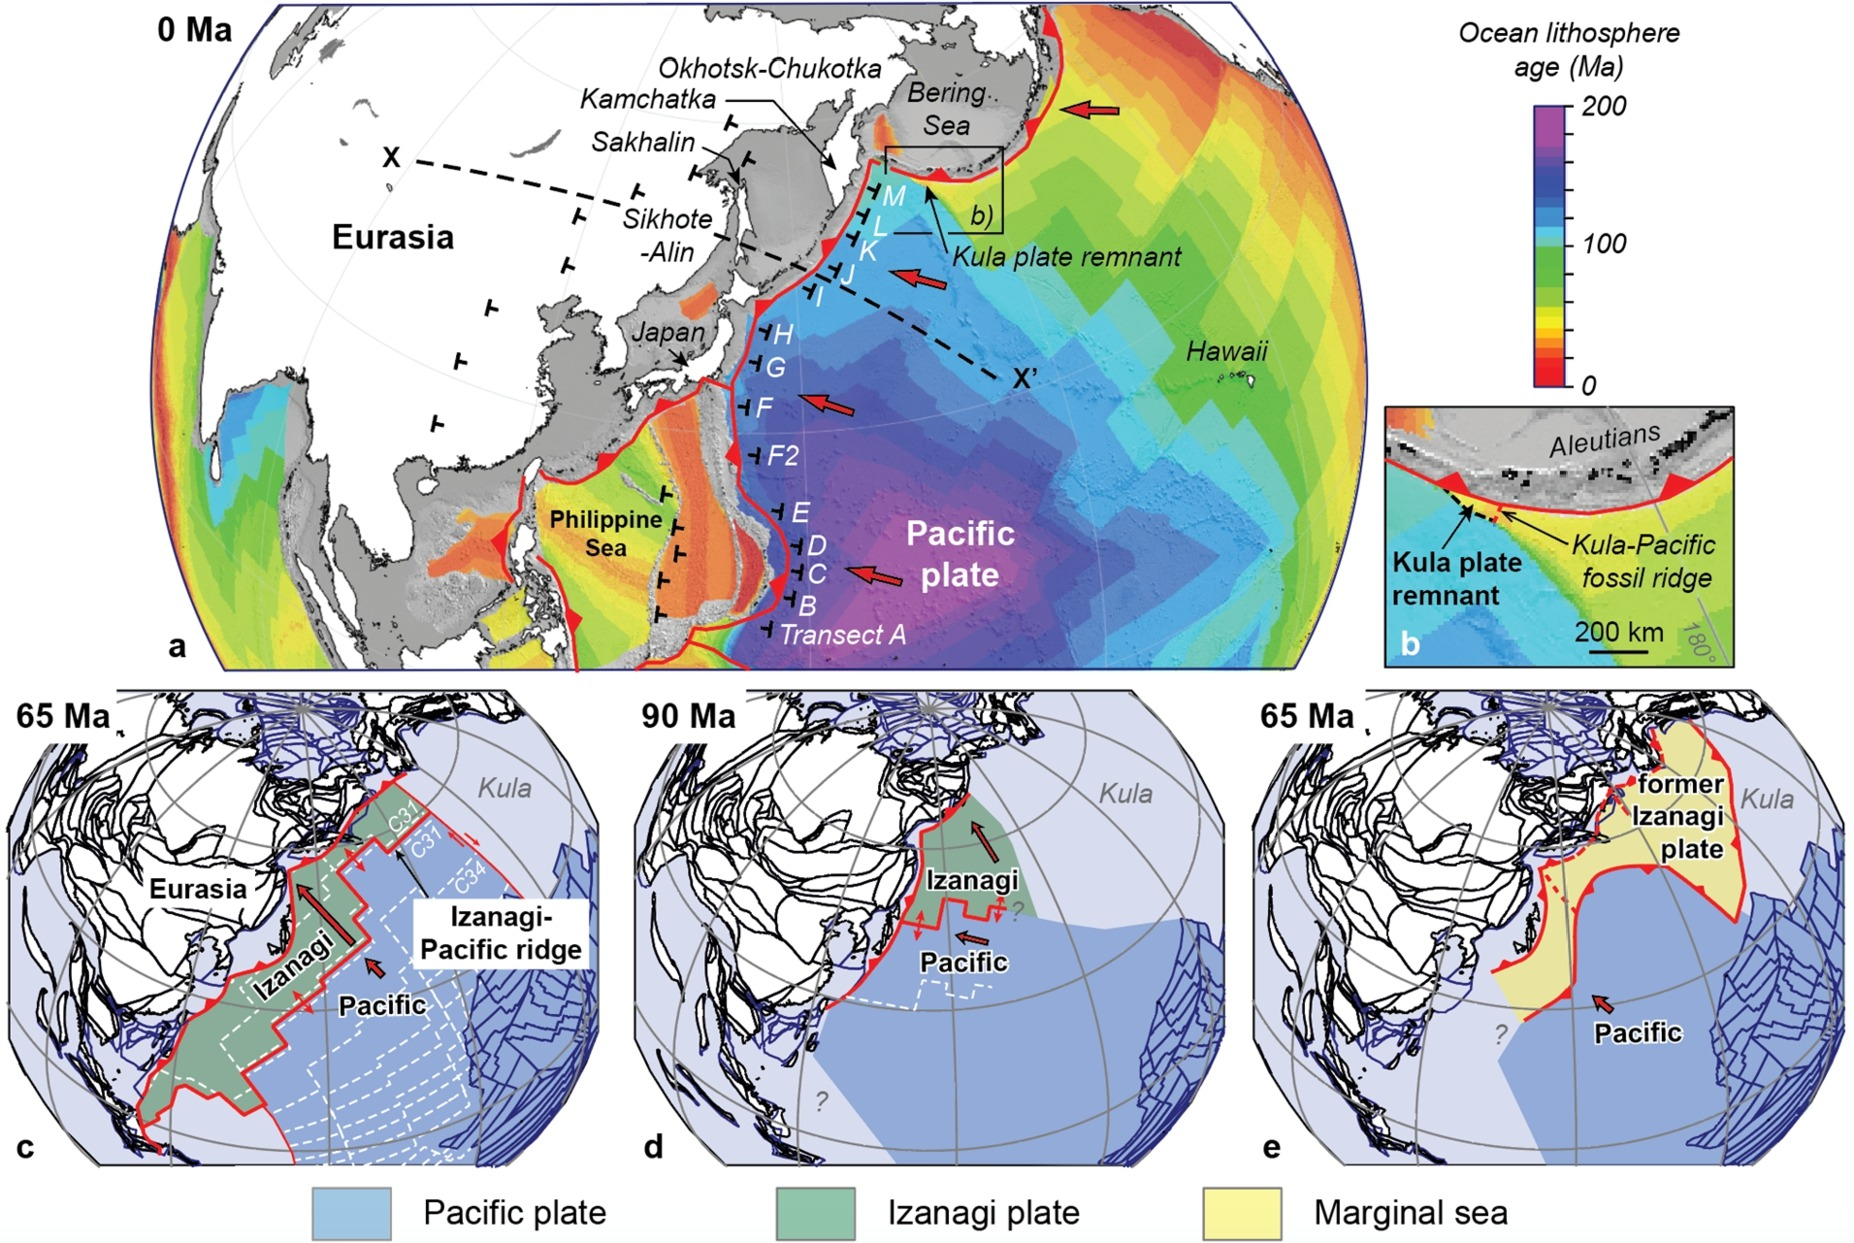
\includegraphics[scale=1.4]{fig/fig02.jpg}%
	\end{adjustbox}
\end{figure}
